\documentclass[authoryear,a4paper,12pt,oneside]{report}
\pagestyle{headings}

% Note that the line below could be modified to suit a
% particular system since the "geometry" package behaves
% differently in Unix, Windows and Mac, especially for the
% top margins.
% Adjust the parameter "top" (measuring the height of the
% space allocated to a header) and "headsep" (measuring
% the distance from the bottom of the header to the
% first line of text.
%\usepackage[top=2.5cm,left=3.8cm,bottom=2.5cm,right=2.5cm,headsep=0.2in]{geometry}

\usepackage{setspace}
%\renewcommand{\baselinestretch}{1.5}


\doublespacing

% Headers and footers for thesis
\usepackage{fancyhdr}

\markboth{}{}
\newcommand\startchapter[1]{\chapter{#1}\thispagestyle{myheadings}}
\newcommand\startappendix[1]{\chapter{#1}\thispagestyle{myheadings}}
\newcommand\startfirstchapter[1]{\chapter{#1}}

% Manual addition of section to Table of Contents
\newcommand\TOCadd[1]{\newpage\phantomsection\addcontentsline{toc}{chapter}{#1}}

% Float Customization
\renewcommand{\floatpagefraction}{0.01}

% Customization of Tables of Contents and List of Figures/Tables
\usepackage[labelsep=space]{caption}

%\usepackage{tocloft}
\usepackage[titles,subfigure]{tocloft}

\renewcommand{\cftchappresnum}{Chapter\ }
\renewcommand\cftchapnumwidth{1.15in}
\makeatletter
\newcommand*\updatechaptername{%
   \addtocontents{toc}{\protect\renewcommand*\protect\cftchappresnum{\@chapapp\ }}
   } \makeatother
\renewcommand\cfttabpresnum{Table\ }
\renewcommand\cfttabnumwidth{0.75in}
\renewcommand\cftfigpresnum{Figure\ }
\renewcommand\cftfignumwidth{1in}





\usepackage{appendix}

%bib format
\usepackage[sort&compress,comma,square,numbers]{natbib}

% Long Table and decimal aligned columns
\usepackage{dcolumn}
\usepackage{longtable}
\usepackage{multirow}

\usepackage{morefloats}


% Mathematics support
\usepackage{amsmath}
\usepackage{amsthm}
\usepackage{amssymb}


% Text Control
\usepackage{xspace}
\usepackage{textcase}
%\usepackage{txfonts}

% Graphics
\usepackage{wasysym}
\usepackage{graphics}
\usepackage{graphicx}   % A package to allow insertion of
                        % external image files
\usepackage{rotating}
\usepackage{subfigure}

%text colour
\usepackage{color}

%\usepackage[colorlinks,linkcolor=black,anchorcolor=black,citecolor=black]{hyperref}   
%bookmarks
\usepackage{setspace}


%==============================================================


\usepackage[BoldFont, SlantFont, CJKchecksingle]{xeCJK}
\setmainfont{Times New Roman}
\setCJKmainfont[Mapping=tex-text]{STKaiti}
\setCJKsansfont[Mapping=tex-text]{KaiTi}
\setCJKmonofont[Mapping=tex-text]{KaiTi}

\usepackage{hyperref}
\usepackage{wallpaper}
\usepackage{graphicx}
\usepackage{amsmath}
\usepackage[final]{pdfpages}
%\usepackage{algorithm}
\usepackage{algorithmicx}
\usepackage{algpseudocode}
\usepackage{multirow}
\usepackage{threeparttable}
\usepackage{enumerate}
\usepackage{adjustbox}
\usepackage{rotating}
%\usepackage{cite}
\usepackage{setspace}
\usepackage{indentfirst}
\usepackage{natbib}
\usepackage{apalike}
\usepackage{setspace}
\usepackage{subfigure}
\usepackage[top=2.5cm,left=3.8cm,bottom=2.5cm,right=2.5cm,headsep=0.2in]{geometry}



\usepackage{caption}
\usepackage[ruled,linesnumbered]{algorithm2e}
\usepackage{algpseudocode}
\makeatletter
\newcommand{\removelatexerror}{\let\@latex@error\@gobble}
\makeatother

\usepackage{amsmath}
\usepackage{multirow}
\usepackage{tabularx}

\usepackage{wallpaper}
\usepackage{graphicx}
\usepackage{amsmath}
\usepackage{pdfpages}
%\usepackage{algorithm}
%\usepackage{algorithmic}
\usepackage{multirow}
\usepackage{threeparttable}
\usepackage{enumerate}
\usepackage{amsmath, amsfonts, amsthm, amssymb, amscd, verbatim, enumerate, bm}
\usepackage{amsthm}
\usepackage{longtable}
\usepackage{graphicx}
\usepackage{multicol}
\usepackage{multirow}
\usepackage{hyperref}
\usepackage{pifont}
\usepackage{booktabs}
\usepackage[font={small}]{caption}
\usepackage{stfloats}
\usepackage{booktabs}
\usepackage{multicol}
\usepackage{url}
\usepackage{amsmath}
\usepackage{multirow}
\usepackage{tabularx}

\usepackage{makecell}
\usepackage[table,xcdraw]{xcolor}

\usepackage{flowchart}
%设置文献的样式

\usepackage{apalike}
\bibliographystyle{apalike} 
\setcitestyle{round,aysep={,},yysep={;}}

%=============================================================
\hypersetup{
    bookmarks=true,         % show bookmarks bar?
    unicode=false,          % non-Latin characters in Acrobat?s bookmarks
%    pdftoolbar=true,        % show Acrobat?s toolbar?
%    pdfmenubar=true,        % show Acrobat?s menu?
%    pdffitwindow=false,     % window fit to page when opened
%    pdfstartview={FitH},    % fits the width of the page to the window
%    pdftitle={My title},    % title
%    pdfauthor={Author},     % author
%    pdfsubject={Subject},   % subject of the document
%    pdfcreator={Creator},   % creator of the document
%    pdfproducer={Producer}, % producer of the document
%    pdfkeywords={keyword1} {key2} {key3}, % list of keywords
%    pdfnewwindow=true,      % links in new window
    colorlinks=true,       % false: boxed links; true: colored links
    linkcolor=blue,          % color of internal links (change box color with linkbordercolor)
    citecolor=blue,        % color of links to bibliography
    %filecolor=magenta,      % color of file links
    %urlcolor=cyan           % color of external links
}

%\floatname{algorithm}{Algorithm}
\renewcommand{\algorithmicrequire}{\textbf{Input:}}
\renewcommand{\algorithmicensure}{\textbf{Output:}}
\renewcommand {\thetable} {\thechapter{}-\arabic{table}} 
\renewcommand {\thefigure} {\thechapter{}.\arabic{figure}}

\newtheorem*{thm}{Theorem}
\setlength{\parindent}{2em}

%==============================================================

%=============================================================
\usepackage{titlesec}

\newcommand{\chaptersize}{\fontsize{18pt}{\baselineskip}\selectfont}
\newcommand{\sectionsize}{\fontsize{16pt}{\baselineskip}\selectfont}
\newcommand{\subsectionsize}{\fontsize{14pt}{\baselineskip}\selectfont}
\newcommand{\chinesesize}{\fontsize{14pt}{\baselineskip}\selectfont}
\newcommand{\chinesechaptersize}{\fontsize{22pt}{\baselineskip}}
\renewcommand\bibname{Reference}

\titleformat{\chapter}{\centering\chaptersize\bfseries}{Chapter\,\thechapter}{1em}{}
\titleformat{\section}{\sectionsize\bfseries}{\thesection}{1em}{}
\titleformat{\subsection}{\itshape\subsectionsize\bfseries}{\thesubsection}{1em}{}
\titlespacing{\chapter}{0pt}{0em}{1em}[0pt]
\titlespacing{\section}{0pt}{2em}{1em}[0pt]
\titlespacing{\subsection}{0pt}{1em}{0em}[0pt]

%==============================================================



\begin{document}
\begin{spacing}{1.0}
\CenterWallPaper{.50}{images/must-logo.jpg}

\pagenumbering{Roman}
\newpage
\thispagestyle{empty}    % Suppress numbers on the first page
\vspace*{1cm}

\begin{center}
\begin{tabular}{p{2cm}p{12cm}}
    \chinesechaptersize{題目:}& \chaptersize{論文的繁體題目}\\
    \;&\;\\
    \;&\;\\
    \chaptersize{Title:} & \chaptersize{Traditional title of the paper}
    \end{tabular}
    \end{center}


    \vspace{2cm}



\begin{center}
    \begin{tabular}{p{2.1cm}p{0.1cm}<{\centering}p{6cm}<{\centering}}
    姓\;\;\;名 & \multirow{2}{*}{:} & \multirow{2}{*}{名\;\;\;字}\\
    Name\\
    \cline{3-3}

    學\;\;\;號 & \multirow{2}{*}{:} & \multirow{2}{*}{190985XX-II20-00XX}\\
    Student No.\\
    \cline{3-3}

    學\;\;\;院 & \multirow{2}{*}{:} & \multirow{2}{*}{資訊科技學院}\\
    Faculty\\
    \cline{3-3}

    課程 & \multirow{2}{*}{:} & \multirow{2}{*}{理學硕士(資訊科技)學位}\\
    Program\\
    \cline{3-3}

    專業 & \multirow{2}{*}{:} & \multirow{2}{*}{計算機與資訊系統}\\
    Major\\
    \cline{3-3}

    指導老師 & \multirow{2}{*}{:} & \multirow{2}{*}{导师名字}\\
    Supervisior\\
    \cline{3-3}

    日期 & \multirow{2}{*}{:} & \multirow{2}{*}{May,2020}\\
    Date\\
    \cline{3-3}

    \end{tabular}

    \end{center}

% \clearpage
% \phantom{s}
% \thispagestyle{empty}


\thispagestyle{empty} 
\vspace{-2.5cm}
\hspace{-3.8cm}
\includepdf{other_pages/declaration.pdf}

\newpage
\setcounter{page}{1}
\TOCadd{摘\;\;要}
\pagestyle{fancy}
\lhead{}
\rhead{\footnotesize{摘\;\;要}}
\vspace*{0.4cm}
\begin{center}

    {\chinesechaptersize{\textbf{摘\;\;要}} \par}
    \vspace*{0.2cm}
\end{center}


\begin{spacing}{1.5}
{\doublespacing
\fontsize{14pt}{\baselineskip}{
	這裏寫中文摘要,要用繁體。

\vspace{2em}
\par \noindent\fontsize{14pt}{\baselineskip}\textbf{關鍵詞}:關鍵詞1, 關鍵詞2, 關鍵詞3
}

}
\end{spacing}

\newpage
\TOCadd{Abstract}
\pagestyle{fancy}
%\lhead{\footnotesize{Orthogonal Representation of Multi-Objects Shape: \\Algorithms and Applications}}
\lhead{}
\rhead{\footnotesize{Abstract}}
\vspace*{0.3cm}
\begin{center}

    {\chaptersize{\textbf{Abstract}} \par}

\end{center}

\begin{spacing}{1.0}
	Write your English abstract here

\vspace{2em}
\par \noindent\textbf{Keywords}:Keywords1, Keywords2, Keywords3
\end{spacing} 
\newpage
\fancypagestyle{plain}{%
\fancyhf{}
\fancyhead[R]{{\footnotesize Contents}}
\fancyfoot[C]{\thepage}
\renewcommand{\headrulewidth}{0.7pt}
\renewcommand{\footrulewidth}{0pt}
}

\pagestyle{fancy}
\lhead{}
\rhead{{\footnotesize Contents}}
\setcounter{lofdepth}{2}{
\TOCadd{Table of Contents}
\tableofcontents

\thispagestyle{fancy}
\lhead{}
\rhead{{\footnotesize Contents}}
\newpage
\fancypagestyle{plain}{%
\fancyhf{}
\fancyhead[R]{{\footnotesize List of Figures}}
\fancyfoot[C]{\thepage}
\renewcommand{\headrulewidth}{0.7pt}
\renewcommand{\footrulewidth}{0pt}
}
\TOCadd{List of Figures}
\pagestyle{fancy}
\lhead{}
\rhead{{\footnotesize List of Figures}}
\setcounter{lofdepth}{1}{
\listoffigures
}
\thispagestyle{fancy}
\lhead{}
\rhead{{\footnotesize List of Figures}}
\newpage
\fancypagestyle{plain}{%
\fancyhf{}
\fancyhead[R]{{\footnotesize List of Tables}}
\fancyfoot[C]{\thepage}
\renewcommand{\headrulewidth}{0.7pt}
\renewcommand{\footrulewidth}{0pt}
}
\TOCadd{List of Tables}
\pagestyle{fancy}
\lhead{}
\rhead{{\footnotesize List of Tables}}
\setcounter{lofdepth}{1}{
\listoftables
}
\thispagestyle{fancy}
\lhead{}
\rhead{{\footnotesize List of Tables}}

\newpage
\pagenumbering{arabic}
\pagestyle{fancy}

\lhead{}
\rhead{\footnotesize{Write your header}}
\chapter{Chapter One}\label{cp1}
\thispagestyle{fancy}


Write your content here.

\section{Section One}
Section1, Section1, Section1, Section1. Here is an example of citing papers for you\citep{lou2020Whole}.


\section{Section Two}
Section2, Section2, Section2, Section2. Here is an example of table for you. Table.\ref{table.1.1}.
\begin{table}[htbp]
	\centering
	\caption{DNA XOR operation}
	\setlength{\tabcolsep}{6.5mm}{
		\begin{tabular}{c|cccc}
			\hline \hline
			XOR   & \textbf{A} & \textbf{T} & \textbf{C} & \textbf{G} \\
			\hline
			\textbf{A} & A     & T     & C     & G \\
			\hline
			\textbf{T} & T     & A     & G     & C \\
			\hline
			\textbf{C} & C     & G     & A     & T \\
			\hline
			\textbf{G} & G     & C     & T     & A \\
			\hline \hline
	\end{tabular}}
	\label{table.1.1}%
\end{table}%
\pagestyle{fancy}
\lhead{}
\rhead{\footnotesize{Write your header}}

\chapter{Chapter Two} \label{cp2}
\thispagestyle{fancy}

Write your content here.

\section{Section One}
Section1,Section1,Section1,Section1. Here is an example of equation for you. Eq.\ref{Eq.2.1}.
\begin{equation}
	\left\{
	\begin{gathered}
		\dot x = a\left( {y - x} \right) \hfill \\
		\dot y = bx - xz - cy + w \hfill \\
		\dot z = xy - dz \hfill \\
		\dot w =  - ky - rw \hfill \\ 
	\end{gathered}
	\right.
	\label{Eq.2.1}
\end{equation}


\section{Section Two}
Section2,Section2,Section2,Section2. Here is an example of figure for you. Fig.\ref{fig.2.1}.
\begin{figure}
	\centering
	
\includegraphics[scale=0.6]{Figs/example.jpg}
	\caption{Example.}
	\label{fig.2.1}
\end{figure}



\newpage

\TOCadd{Reference}
\fancypagestyle{plain}{%
\fancyhf{}
\fancyhead[R]{{\footnotesize Reference}}
\fancyfoot[C]{\thepage}
\renewcommand{\headrulewidth}{0.7pt}
\renewcommand{\footrulewidth}{0pt}
}
\pagestyle{fancy}
\lhead{}
\rhead{{\footnotesize Reference}}
\bibliographystyle{apalike}
%\bibliographystyle{tJDE}
\bibliography{bibliography.bib}  % Quote the bibliography.bib in Folder bibfile
\thispagestyle{fancy}
\lhead{}
\rhead{{\footnotesize Reference}}







\newpage
\addcontentsline{toc}{chapter}{Acknowledgements}
\begin{center}
\thispagestyle{fancy}
\lhead{}
\rhead{\small Acknowledgements}
    \setlength{\parskip}{0pt}
    {\bf\Large{Acknowledgements} \par}
    \bigskip
\end{center}

\par Write down your Acknowledgements here, and don't forget the credit of this template, although it is not very good.


\TOCadd{Personal Resume}
\pagestyle{fancy}
\lhead{}
\rhead{\footnotesize{Personal Resume}}


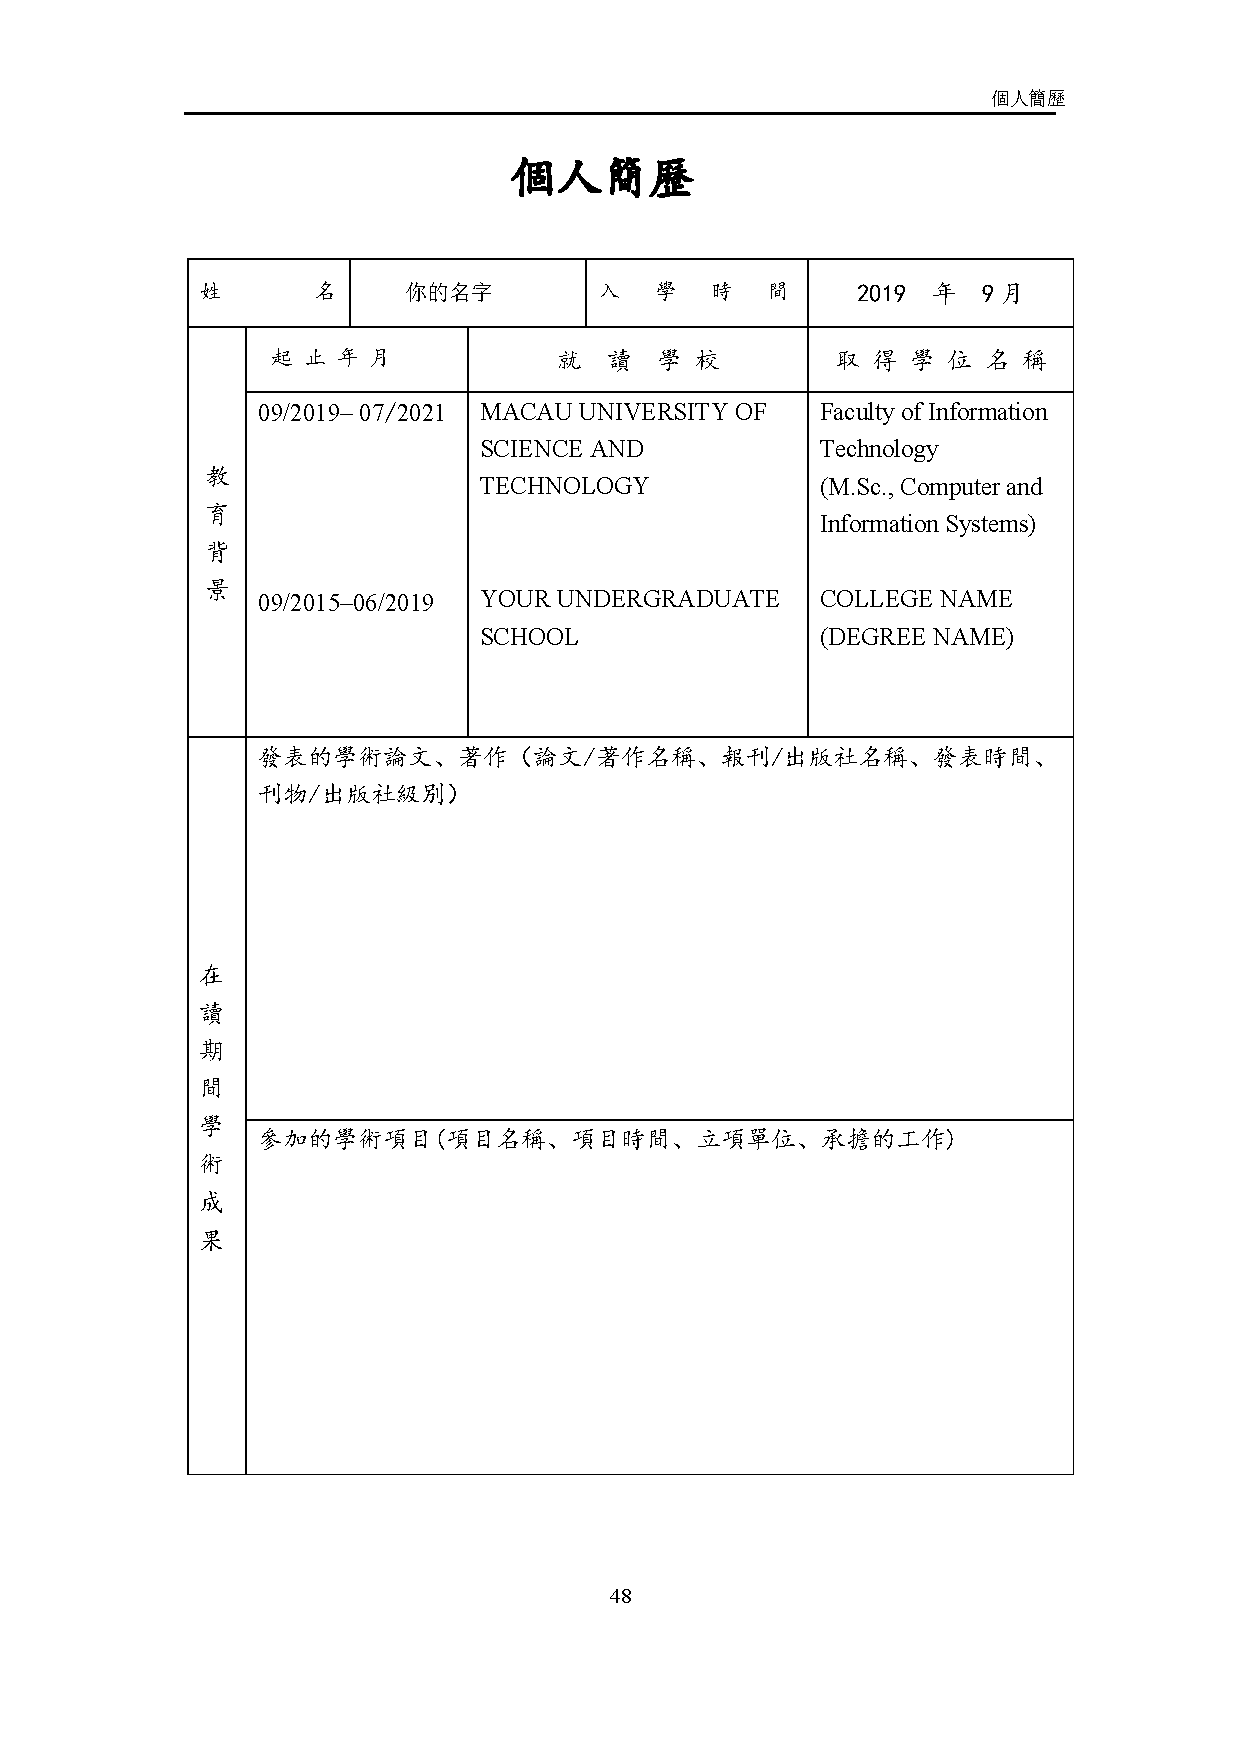
\includepdf{other_pages/personal_resume.pdf}

%\begin{figure}[htbp]
%\centering
%\includegraphics[scale=0.34]{frontmatter/per.jpg}
%\end{figure}


}\end{spacing}
\end{document}
